%=====================================================================
%  How the Kungsgatan and Slottsgatan Vissim model works
%  A plain-language guide to the model, its inputs and its behaviour
%
%  Every number in this document was read from the model files:
%    Vissim_lab.inpx, Fixed_time.sig, Signal_data.pua,
%    Control_logic.vap / .vv, traffic_measurements.xlsx
%
%  Figures expected in the same folder (upload to Overleaf):
%    fig_network.png   fig_residuals.png
%  All other diagrams are drawn with TikZ / pgfplots and need no file.
%=====================================================================
\documentclass[11pt,a4paper]{article}

\usepackage[utf8]{inputenc}
\usepackage[T1]{fontenc}
\usepackage{lmodern}
\usepackage{microtype}
\usepackage[margin=2.4cm,headheight=14pt]{geometry}
\usepackage{amsmath,amssymb}
\usepackage{booktabs}
\usepackage{graphicx}
\usepackage{array}
\usepackage{tabularx}
\usepackage[table]{xcolor}
\usepackage{caption}
\usepackage{enumitem}
\usepackage{fancyhdr}
\usepackage[most]{tcolorbox}
\usepackage{tikz}
\usetikzlibrary{arrows.meta,positioning,calc,shapes.geometric}
\usepackage{pgfplots}
\pgfplotsset{compat=1.18}
\usepackage[hidelinks]{hyperref}
\usepackage[capitalise,noabbrev]{cleveref}

%---------------------------------------------------------------------
% Style
%---------------------------------------------------------------------
\definecolor{accent}{HTML}{1F5FA8}
\definecolor{lightaccent}{HTML}{E8F0FA}
\definecolor{sgreen}{HTML}{2E9E44}
\definecolor{samber}{HTML}{E8A317}
\definecolor{sred}{HTML}{C62828}
\definecolor{road}{HTML}{BFC5CC}

\captionsetup{font=small,labelfont={bf,color=accent},labelsep=period}
\setlist{itemsep=2pt,topsep=4pt}
\renewcommand{\arraystretch}{1.12}

\pagestyle{fancy}
\fancyhf{}
\fancyhead[L]{\small\textcolor{gray}{How the Kungsgatan and Slottsgatan Vissim model works}}
\fancyhead[R]{\small\textcolor{gray}{M.\,N.\ Tabassum}}
\fancyfoot[C]{\small\thepage}
\renewcommand{\headrulewidth}{0.3pt}

\newtcolorbox{keybox}[1]{colback=lightaccent,colframe=accent,fonttitle=\bfseries,
  title={#1},boxrule=0.6pt,arc=2pt,left=6pt,right=6pt,top=4pt,bottom=4pt}
\newtcolorbox{plainbox}[1]{colback=white,colframe=accent!60,fonttitle=\bfseries\color{accent},
  coltitle=accent,colbacktitle=white,title={#1},boxrule=0.5pt,arc=2pt,left=6pt,right=6pt}

\newcommand{\code}[1]{\texttt{#1}}
\newcommand{\kmh}{~km/h}
\newcommand{\vph}{~veh/h}

%=====================================================================
\begin{document}
%=====================================================================

\begin{titlepage}
\thispagestyle{empty}
\centering
\vspace*{2.4cm}
{\color{accent}\rule{\textwidth}{1.2pt}}\\[14pt]
{\LARGE\bfseries How the Kungsgatan and Slottsgatan\\[4pt] Vissim Model Works\par}
\vspace{10pt}
{\large A plain-language guide to the model, its inputs,\\ its behaviour and its results\par}
\vspace{10pt}
{\color{accent}\rule{\textwidth}{1.2pt}}\\[2cm]
{\Large Muhammad Noman Tabassum\par}
\vspace{8pt}
{\large Infra Informatics PhD course\\ Simulation module, Vissim lab\par}
\vfill
\begin{tabular}{@{}ll@{}}
\toprule
Model file & \code{Vissim\_lab.inpx} (PTV Vissim) \\
Signal files & \code{Fixed\_time.sig}, \code{Control\_logic.vap}, \code{Signal\_data.pua} \\
Field data & \code{traffic\_measurements.xlsx} (10 weekday mornings) \\
Location & Kungsgatan and Slottsgatan, Norrk\"oping \\
\bottomrule
\end{tabular}
\vspace{1.6cm}

{\large October 2026\par}
\end{titlepage}

%---------------------------------------------------------------------
\section*{About this document}
\addcontentsline{toc}{section}{About this document}

This document explains, step by step, how the Vissim model of the signalised intersection of
Kungsgatan and Slottsgatan in Norrk\"oping works. It is written for readers who have never used
Vissim: every technical term is explained when it first appears, and a glossary is given at the
end (\cref{sec:glossary}). Readers who know Vissim will find the exact object numbers and parameter
values in the tables.

Every number in this document was read directly from the model files listed on the title page,
not taken from memory or from general defaults. Where the document gives an estimate rather than a
value from the files, it says so explicitly.

\begin{keybox}{The model at a glance}
\begin{tabularx}{\linewidth}{@{}>{\bfseries}p{3.6cm}X@{}}
What it represents & One four-armed signalised intersection in central Norrk\"oping: Kungsgatan
(north to south) crossing Slottsgatan (east to west).\\
Road users & Cars (95\,\%) and heavy goods vehicles (5\,\%), bicycles and e-bikes on two cycle
tracks along Kungsgatan, pedestrians on four crosswalks.\\
Demand & 2\,150 motor vehicles, 200 cyclists and 170 pedestrians per hour, constant over time.\\
Signal control & Fixed-time, two stages, 90-second cycle (an actuated alternative is included).\\
How it works & Every road user is simulated individually, ten times per simulated second.\\
What it measures & Speeds and accelerations at 12 points, queue lengths at 10 points, and the
average delay of all vehicles.\\
Simulated time & 30 minutes (1\,800~s) per run in the original file.\\
\end{tabularx}
\end{keybox}

\tableofcontents
\newpage

%=====================================================================
\section{What is a microscopic traffic simulation?}
\label{sec:micro}
%=====================================================================

A \emph{microscopic} traffic simulation represents every single road user (every car, truck,
bicycle and pedestrian) as an individual object with its own position, speed, destination and
personal driving style. This is different from \emph{macroscopic} models, which describe traffic
as a flow, like water in a pipe, without individual vehicles.

PTV Vissim, the software used here, moves time forward in small, equal steps. In this model the
\emph{simulation resolution} is 10 time steps per simulated second, so the simulation advances in
steps of 0.1~s. In every step, each road user looks at its surroundings and decides how to move
(\cref{fig:loop}):

\begin{figure}[!htb]
\centering
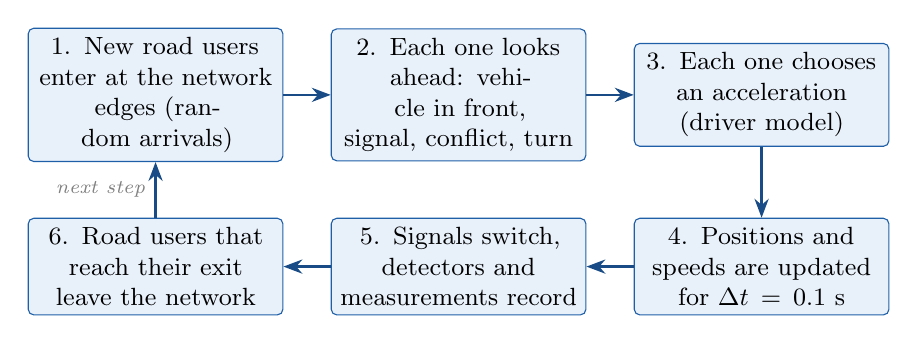
\begin{tikzpicture}[
  node distance=5mm and 6mm,
  box/.style={draw=accent, fill=lightaccent, rounded corners=2pt, align=center,
              minimum height=12mm, text width=30mm, font=\small},
  arr/.style={-{Stealth[length=2.4mm]}, thick, accent!80!black}]
\node[box] (a) {1. New road users\\enter at the network\\edges (random arrivals)};
\node[box, right=of a] (b) {2. Each one looks\\ahead: vehicle in front,\\signal, conflict, turn};
\node[box, right=of b] (c) {3. Each one chooses\\an acceleration\\(driver model)};
\node[box, below=9mm of c] (d) {4. Positions and\\speeds are updated\\for $\Delta t = 0.1$~s};
\node[box, left=of d] (e) {5. Signals switch,\\detectors and\\measurements record};
\node[box, left=of e] (f) {6. Road users that\\reach their exit\\leave the network};
\draw[arr] (a) -- (b);
\draw[arr] (b) -- (c);
\draw[arr] (c) -- (d);
\draw[arr] (d) -- (e);
\draw[arr] (e) -- (f);
\draw[arr] (f.north) -- node[left, font=\scriptsize\itshape, text=gray]{next step} (a.south);
\end{tikzpicture}
\caption[What happens in every simulation step]{What happens in every simulation step of 0.1~s.
One simulated half hour therefore consists of 18\,000 such steps.}
\label{fig:loop}
\end{figure}

\paragraph{Randomness.} Real traffic is never the same twice: drivers arrive at random moments and
have different preferences. Vissim reproduces this with random numbers. Arrival times, each
driver's preferred speed and each driver's personal following distance are drawn at random from
statistical distributions. The sequence of random numbers is controlled by a \emph{random seed}:
the same model with the same seed always gives exactly the same result, while a different seed
gives a different, equally plausible half hour of traffic. One simulation with one seed is called
a \emph{run} or \emph{replication}. Because a single run is only one possible outcome, results
are always averaged over several runs with different seeds (\cref{sec:running}).

%=====================================================================
\section{The road network}
\label{sec:network}
%=====================================================================

\subsection{Links and connectors}

In Vissim, roads are drawn as \emph{links}: directed strips with one or more lanes on which road
users travel in one direction only. Links are joined by \emph{connectors}, short curved pieces that
carry road users from the end of one link onto another link. All turning movements inside the
intersection are connectors. The model contains 22 links and 16 connectors
(\cref{tab:links}). The network is drawn for right-hand traffic.

\begin{table}[!htb]
\centering
\caption[Links of the model]{The 22 links of the model. ``Behaviour'' is the link behaviour type,
which decides how road users on that link interact (\cref{sec:behaviour}). Lengths are measured
from the link geometry in the file.}
\label{tab:links}
\small
\begin{tabularx}{\textwidth}{lXlrr}
\toprule
\textbf{Link} & \textbf{Role} & \textbf{Behaviour} & \textbf{Width} & \textbf{Length}\\
\midrule
2  & Kungsgatan northbound, from the south edge through the junction to the north edge & Urban & 3.0~m & 131~m\\
4  & Kungsgatan southbound, from the north edge through the junction to the south edge & Urban & 3.0~m & 115~m\\
5  & Slottsgatan westbound approach (traffic arriving from the east)  & Urban & 3.0~m & 59~m\\
11 & Slottsgatan eastbound approach (traffic arriving from the west)  & Urban & 3.0~m & 63~m\\
1  & Slottsgatan exit towards the east  & Urban & 3.0~m & 68~m\\
3  & Slottsgatan exit towards the west  & Urban & 3.0~m & 63~m\\
6, 8, 7, 12 & Left-turn pockets of the northbound, southbound, westbound and eastbound approaches
& Urban & 3.0~m & 30 to 37~m\\
9, 10, 13 to 18 & Pedestrian crosswalks, two directions on each of the four arms & Footpath & 1.5~m & 14 to 15~m\\
19 to 22 & Cycle tracks along Kungsgatan, two per direction (before and after the junction) & Cycle track & 1.5~m & 58 to 63~m\\
\bottomrule
\end{tabularx}
\end{table}

Every motorised approach has a single lane of 3~m. A short \emph{left-turn pocket} branches off
each approach some 10 to 20~m after the network edge, so that vehicles waiting to turn left do not
block vehicles going straight or turning right. Kungsgatan is modelled as two continuous links
(2 and 4) that run straight through the junction; Slottsgatan ends at the junction on each side and
continues on separate exit links (1 and 3). \Cref{fig:network} shows the network as drawn from the
coordinates in the file, together with the measurement points described in \cref{sec:measure}.

\begin{figure}[!htb]
\centering
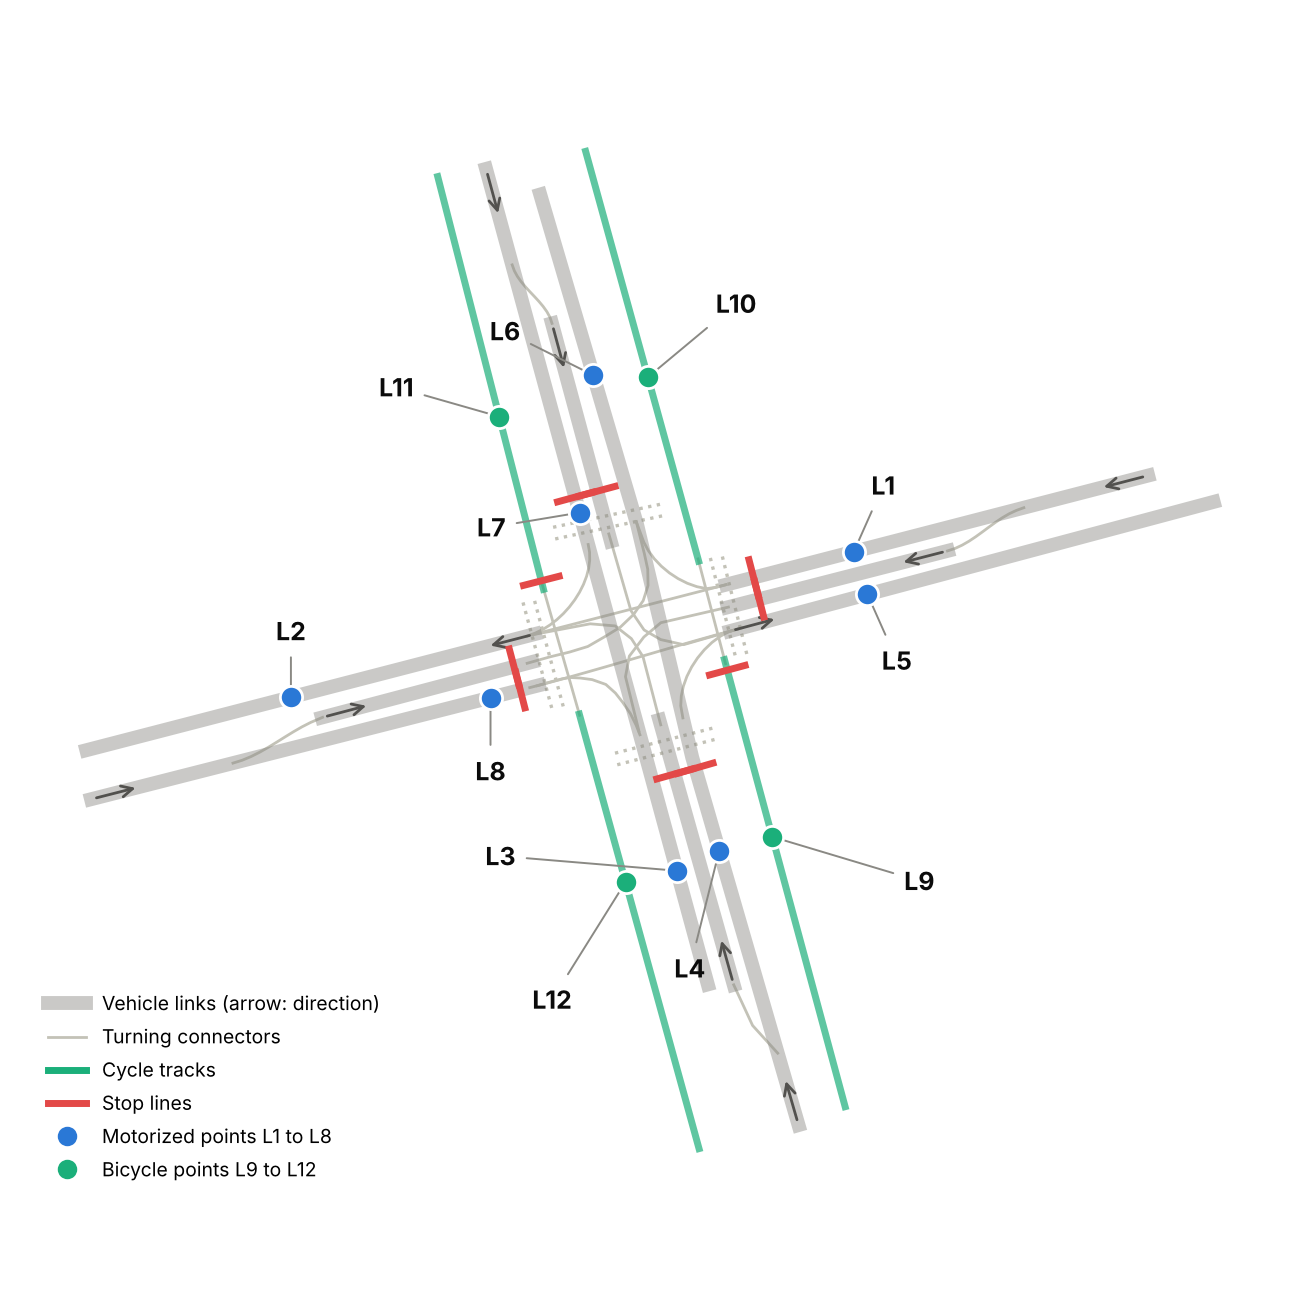
\includegraphics[width=0.8\textwidth]{fig_network.png}
\caption[The Vissim network]{The Vissim network: links, turning connectors, stop lines and the
twelve data collection points L1 to L12, plotted from the coordinates in \code{Vissim\_lab.inpx}.}
\label{fig:network}
\end{figure}

\subsection{Turning movements}

The 16 connectors create every possible movement through the junction. Right turns and the
straight movements on Slottsgatan go directly from the approach to the exit; left turns go from
the approach into the left-turn pocket and from there across the junction
(\cref{tab:movements}). The two cycle tracks only go straight.

\begin{table}[!htb]
\centering
\caption[Movements and the connectors that carry them]{Movements and the connectors that carry
them (connector numbers as in the model file).}
\label{tab:movements}
\footnotesize
\setlength{\tabcolsep}{4pt}
\begin{tabular}{llll}
\toprule
\textbf{Approach} & \textbf{Left} & \textbf{Straight} & \textbf{Right}\\
\midrule
Kungsgatan northbound (2)  & 10003, pocket 6, 10006 to west   & link 2 continues & 10000 to east\\
Kungsgatan southbound (4)  & 10010, pocket 8, 10009 to east   & link 4 continues & 10007 to west\\
Slottsgatan westbound (5)  & 10002, pocket 7, 10005 to south  & 10001 to west    & 10004 to north\\
Slottsgatan eastbound (11) & 10013, pocket 12, 10012 to north & 10011 to east    & 10008 to south\\
Cycle tracks (20, 22)      &                                  & 10014, 10015     & \\
\bottomrule
\end{tabular}
\end{table}

%=====================================================================
\section{Who uses the network: traffic demand}
\label{sec:demand}
%=====================================================================

\subsection{Types of road users}

Vissim groups road users into \emph{vehicle types}, which are collected in \emph{vehicle classes}.
\Cref{tab:types} lists the types that actually appear in this model. Pedestrians are modelled in a
simple way, as a special vehicle type that walks on the crosswalk links.

\begin{table}[!htb]
\centering
\caption[Road user types in the model]{Road user types that appear in the model.}
\label{tab:types}
\small
\begin{tabular}{lllll}
\toprule
\textbf{Class} & \textbf{Type (number)} & \textbf{Where} & \textbf{Share} & \textbf{Desired speed}\\
\midrule
Car (10)        & Car (100)    & all motorised inputs & 95\,\% & uniform 48 to 58\kmh\\
HGV (20)        & HGV (200)    & all motorised inputs & 5\,\%  & uniform 48 to 58\kmh\\
Bike (60)       & Bike (610)   & both cycle tracks    & 80\,\% & uniform 12 to 15\kmh\\
Bike (60)       & E-bike (620) & both cycle tracks    & 20\,\% & uniform 15 to 20\kmh\\
Pedestrian (50) & Man (510)    & all crosswalks       & 100\,\% & uniform 4 to 6\kmh\\
\bottomrule
\end{tabular}
\end{table}

\subsection{How road users enter the model}

Road users are created at \emph{vehicle inputs}, placed at the start of each link that enters the
network. An input has a volume in road users per hour and a \emph{vehicle composition}, which says
which types arrive and in what proportions. The arrivals are \emph{stochastic}: the input produces
the stated number per hour on average, but the exact moments of arrival are random, as in reality.
The model has 14 inputs (\cref{tab:inputs}). The volumes are defined for three consecutive
15-minute intervals with identical values, so the demand is constant over the simulated period.

\begin{table}[!htb]
\centering
\caption[Vehicle inputs]{Vehicle inputs of the model. Letters A, C, E and G are the names used in
the lab instructions.}
\label{tab:inputs}
\small
\begin{tabularx}{\textwidth}{r>{\raggedright\arraybackslash}Xlr>{\raggedright\arraybackslash}p{3.4cm}}
\toprule
\textbf{Input} & \textbf{Location} & \textbf{Link} & \textbf{Per hour} & \textbf{Composition}\\
\midrule
1  & A: Kungsgatan from the north (southbound) & 4  & 660   & Default (95\,\% car, 5\,\% HGV)\\
3  & E: Kungsgatan from the south (northbound) & 2  & 1\,040 & Default\\
4  & C: Slottsgatan from the east (westbound)  & 5  & 240   & Default\\
11 & G: Slottsgatan from the west (eastbound)  & 11 & 210   & Default\\
14, 15 & Cycle tracks, north- and southbound   & 20, 22 & 100 each & Bike (80\,\% bike, 20\,\% e-bike)\\
5, 6   & Crosswalk on the south arm, both directions & 13, 14 & 25 each & Ped\\
7 to 10, 12, 13 & Crosswalks on the other three arms & 9, 10, 15 to 18 & 20 each & Ped\\
\bottomrule
\end{tabularx}
\end{table}

\subsection{Where they go: routes}

Once a vehicle has entered, a \emph{static routing decision} near the start of the approach assigns
it a route, i.e.\ left, straight or right. The choice is random, with fixed probabilities given by
the relative flows of the routes (\cref{tab:routes}). Multiplying the input volume by these shares
gives the average hourly volume of each movement.

\begin{table}[!htb]
\centering
\caption[Route shares and movement volumes]{Route shares of the four routing decisions and the
resulting average movement volumes (vehicles per hour).}
\label{tab:routes}
\small
\begin{tabular}{lrrrrrrr}
\toprule
& & \multicolumn{3}{c}{\textbf{Share}} & \multicolumn{3}{c}{\textbf{Volume [veh/h]}}\\
\cmidrule(lr){3-5}\cmidrule(lr){6-8}
\textbf{Approach} & \textbf{Input} & \textbf{Left} & \textbf{Straight} & \textbf{Right} & \textbf{Left} & \textbf{Straight} & \textbf{Right}\\
\midrule
Kungsgatan northbound (E) & 1\,040 & 0.08 & 0.75 & 0.17 & 83  & 780 & 177\\
Kungsgatan southbound (A) & 660    & 0.15 & 0.79 & 0.06 & 99  & 521 & 40\\
Slottsgatan westbound (C) & 240    & 0.50 & 0.08 & 0.42 & 120 & 19  & 101\\
Slottsgatan eastbound (G) & 210    & 0.57 & 0.14 & 0.29 & 120 & 29  & 61\\
\bottomrule
\end{tabular}
\end{table}

Kungsgatan carries four fifths of the motor traffic. The heaviest single movement is the 780
vehicles per hour going straight north on Kungsgatan. On Slottsgatan, most vehicles turn; only 8 to
14\,\% go straight across.

\begin{figure}[!htb]
\centering
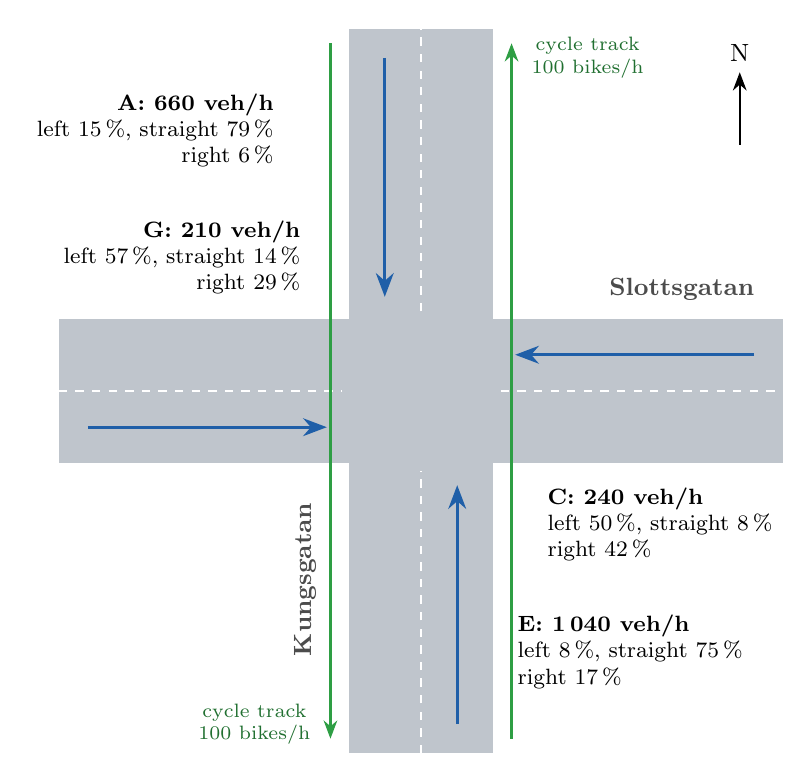
\begin{tikzpicture}[scale=0.92, font=\small]
  % roads
  \fill[road] (-1,-5) rectangle (1,5);
  \fill[road] (-5,-1) rectangle (5,1);
  \draw[white, dashed, thick] (0,-5) -- (0,-1.1) (0,1.1) -- (0,5) (-5,0) -- (-1.1,0) (1.1,0) -- (5,0);
  % street names
  \node[rotate=90, font=\small\bfseries, text=gray!60!black] at (-1.6,-2.6) {Kungsgatan};
  \node[font=\small\bfseries, text=gray!60!black] at (3.6,1.4) {Slottsgatan};
  % compass
  \draw[-{Stealth}, thick] (4.4,3.4) -- (4.4,4.4) node[above]{N};
  % approaches: E northbound (bottom, right lane x>0 going up)
  \draw[-{Stealth[length=3mm]}, very thick, accent] (0.5,-4.6) -- (0.5,-1.3);
  \node[align=left, anchor=west, font=\footnotesize] at (1.2,-3.6)
      {\textbf{E: 1\,040 veh/h}\\left 8\,\%, straight 75\,\%\\right 17\,\%};
  % A southbound (top, left lane x<0 going down)
  \draw[-{Stealth[length=3mm]}, very thick, accent] (-0.5,4.6) -- (-0.5,1.3);
  \node[align=right, anchor=east, font=\footnotesize] at (-1.9,3.6)
      {\textbf{A: 660 veh/h}\\left 15\,\%, straight 79\,\%\\right 6\,\%};
  % C westbound (right side, upper lane y>0 going left)
  \draw[-{Stealth[length=3mm]}, very thick, accent] (4.6,0.5) -- (1.3,0.5);
  \node[align=left, anchor=north, font=\footnotesize] at (3.3,-1.2)
      {\textbf{C: 240 veh/h}\\left 50\,\%, straight 8\,\%\\right 42\,\%};
  % G eastbound (left side, lower lane y<0 going right)
  \draw[-{Stealth[length=3mm]}, very thick, accent] (-4.6,-0.5) -- (-1.3,-0.5);
  \node[align=right, anchor=south, font=\footnotesize] at (-3.3,1.2)
      {\textbf{G: 210 veh/h}\\left 57\,\%, straight 14\,\%\\right 29\,\%};
  % cycle tracks
  \draw[-{Stealth}, thick, sgreen] (1.25,-4.8) -- (1.25,4.8);
  \draw[-{Stealth}, thick, sgreen] (-1.25,4.8) -- (-1.25,-4.8);
  \node[font=\scriptsize, text=sgreen!70!black, align=center] at (2.3,4.6) {cycle track\\100 bikes/h};
  \node[font=\scriptsize, text=sgreen!70!black, align=center] at (-2.3,-4.6) {cycle track\\100 bikes/h};
\end{tikzpicture}
\caption[Schematic of the demand]{Schematic of the demand (not to scale). Blue arrows: motorised
approaches with their hourly volume and turning shares. Green arrows: the two cycle tracks along
Kungsgatan.}
\label{fig:demand}
\end{figure}

%=====================================================================
\section{How road users move}
\label{sec:behaviour}
%=====================================================================

This section describes the rules that decide how each road user accelerates, follows others,
brakes and turns. Together they are called the \emph{driving behaviour}.

\subsection{Desired speed}

Every road user has a \emph{desired speed}: the speed it would choose on an empty road. It is drawn
at random from a \emph{desired speed distribution} when the road user enters the network and kept
for the whole trip. In this model all distributions used for road users are uniform, meaning
every value between the lower and the upper bound is equally likely (\cref{tab:types}). A car
therefore wants to drive somewhere between 48 and 58\kmh, on average 53\kmh. A road user drives
slower than its desired speed only when something forces it to: a vehicle in front, a red signal,
a turn or a conflict.

\subsection{Acceleration and braking}

How quickly a vehicle speeds up or slows down is given by speed-dependent functions. The
\emph{desired acceleration} is what a driver normally uses; the \emph{maximum acceleration} is the
technical limit of the vehicle. Both decrease with speed: a car accelerates strongly from standstill
and more gently near its desired speed (\cref{fig:accel}). Each vehicle also receives its own
random position between a lower and an upper curve, so that some drivers are more dynamic than
others.

For normal braking, cars use a \emph{desired deceleration} of $-2.75$~m/s$^2$ and HGVs
$-1.25$~m/s$^2$, independent of speed. In an emergency, cars can brake up to $-7.5$~m/s$^2$ and
HGVs up to $-5.5$~m/s$^2$ (the \emph{maximum deceleration}).

\begin{figure}[!htb]
\centering
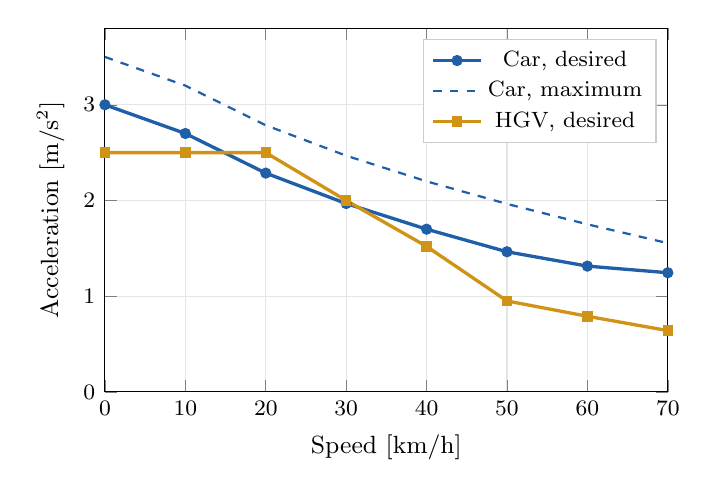
\begin{tikzpicture}
\begin{axis}[
  width=0.72\textwidth, height=6.2cm,
  xlabel={Speed [km/h]}, ylabel={Acceleration [m/s$^2$]},
  xmin=0, xmax=70, ymin=0, ymax=3.8,
  grid=major, grid style={gray!20},
  legend style={font=\footnotesize, at={(0.98,0.97)}, anchor=north east, draw=gray!40},
  tick label style={font=\footnotesize}, label style={font=\small}]
\addplot[very thick, accent, mark=*, mark size=1.4pt] coordinates
  {(0,3.0) (10,2.7) (20,2.286) (30,1.968) (40,1.7) (50,1.464) (60,1.314) (70,1.245)};
\addlegendentry{Car, desired}
\addplot[thick, accent, dashed] coordinates
  {(0,3.5) (10,3.2) (20,2.786) (30,2.468) (40,2.2) (50,1.964) (60,1.751) (70,1.554)};
\addlegendentry{Car, maximum}
\addplot[very thick, samber!90!black, mark=square*, mark size=1.3pt] coordinates
  {(0,2.5) (10,2.5) (20,2.5) (30,2.0) (40,1.52) (50,0.95) (60,0.79) (70,0.64)};
\addlegendentry{HGV, desired}
\end{axis}
\end{tikzpicture}
\caption[Acceleration functions]{Average desired and maximum acceleration as a function of speed,
read from the acceleration functions in the model file.}
\label{fig:accel}
\end{figure}

\subsection{Following the vehicle in front: the Wiedemann 74 model}
\label{sec:w74}

The most important rule is how a vehicle follows the vehicle in front of it. All motorised links
use the driving behaviour \emph{Urban (motorized)}, which applies the car-following model of
Wiedemann (1974), the standard model for urban traffic in Vissim. Its basic idea is that a driver
is always in one of four situations:
\begin{enumerate}
  \item \textbf{Free driving:} nobody close in front; the driver accelerates towards the desired
        speed.
  \item \textbf{Approaching:} a slower vehicle is ahead; the driver slows down to match its speed
        before reaching the safety distance.
  \item \textbf{Following:} the driver follows at about the safety distance, with small,
        unconscious speed fluctuations around the leader's speed.
  \item \textbf{Braking:} the gap has become shorter than the safety distance; the driver brakes
        more strongly to restore it.
\end{enumerate}

The \emph{safety distance} $d$ that a driver wants to keep to the vehicle in front is
\begin{equation}
d = a_x + b_x, \qquad b_x = \left(b_{x,\mathrm{add}} + b_{x,\mathrm{mult}}\cdot z\right)\sqrt{v},
\label{eq:w74}
\end{equation}
where $v$ is the speed in m/s and $z$ is a personal random value of each driver between 0 and 1
(on average 0.5). The three parameters of \cref{eq:w74} are the ones that the lab instructions
suggest for calibration (\cref{tab:w74}).

\begin{table}[!htb]
\centering
\caption[Car-following parameters]{Car-following parameters of driving behaviour 1, Urban
(motorized), as given in the model file.}
\label{tab:w74}
\small
\begin{tabularx}{\textwidth}{lrX}
\toprule
\textbf{Parameter} & \textbf{Value} & \textbf{Meaning}\\
\midrule
$a_x$, average standstill distance & 2.0~m & Gap between two stopped vehicles, e.g.\ in a queue at
a red light.\\
$b_{x,\mathrm{add}}$, additive part of safety distance & 2.0 & Base part of the extra distance
that grows with speed.\\
$b_{x,\mathrm{mult}}$, multiplicative part & 3.0 & Personal part of the extra distance, scaled by
the random value $z$; it makes drivers different from each other.\\
Reduction factor near signals & 0.6 & Within 100~m upstream and 100~m downstream of a signal
head, the safety distance is multiplied by 0.6, because drivers close up when approaching and
leaving a stop line.\\
Look-ahead distance & 0 to 250~m & How far ahead a driver perceives vehicles and signals; up to 4
objects ahead are taken into account.\\
\bottomrule
\end{tabularx}
\end{table}

\begin{plainbox}{Worked example}
A car driving at 50\kmh{} ($v = 13.9$~m/s, $\sqrt{v} = 3.73$) with an average personal value
$z = 0.5$ wants a safety distance of
\[
d = 2.0 + (2.0 + 3.0 \cdot 0.5)\cdot 3.73 = 2.0 + 13.0 = 15.0~\text{m},
\]
which corresponds to a time gap of about 1.1~s. Close to the signal the extra part is reduced to
60\,\%, giving $2.0 + 0.6 \cdot 13.0 \approx 9.8$~m. Smaller safety distances let more vehicles pass
the stop line per second of green, so these parameters directly control the \emph{capacity} of the
intersection.
\end{plainbox}

\begin{figure}[!htb]
\centering
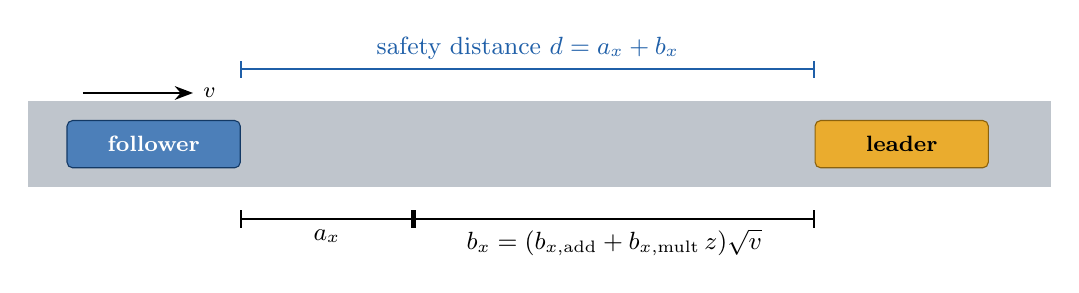
\begin{tikzpicture}[font=\small]
  \fill[road] (-0.5,-0.55) rectangle (12.5,0.55);
  % follower
  \draw[fill=accent!80, draw=accent!60!black, rounded corners=2pt] (0,-0.3) rectangle (2.2,0.3);
  \node[white, font=\footnotesize\bfseries] at (1.1,0) {follower};
  % leader
  \draw[fill=samber!90, draw=samber!60!black, rounded corners=2pt] (9.5,-0.3) rectangle (11.7,0.3);
  \node[font=\footnotesize\bfseries] at (10.6,0) {leader};
  % distances
  \draw[|-|, thick] (2.2,-0.95) -- node[below]{$a_x$} (4.4,-0.95);
  \draw[|-|, thick] (4.4,-0.95) -- node[below]{$b_x = (b_{x,\mathrm{add}} + b_{x,\mathrm{mult}}\, z)\sqrt{v}$} (9.5,-0.95);
  \draw[|-|, thick, accent] (2.2,0.95) -- node[above]{safety distance $d = a_x + b_x$} (9.5,0.95);
  \draw[-{Stealth}, thick] (0.2,0.65) -- (1.6,0.65) node[right, font=\footnotesize]{$v$};
\end{tikzpicture}
\caption[Safety distance in the Wiedemann 74 model]{The safety distance in the Wiedemann 74
car-following model: a fixed standstill part $a_x$ and a part $b_x$ that grows with the square root
of the speed $v$.}
\label{fig:w74}
\end{figure}

\subsection{Cyclists and pedestrians}

Cyclists use the behaviour \emph{Cycle-Track (free overtaking)}, which applies the Wiedemann 99
model with a standstill distance of 0.5~m and allows cyclists to overtake each other within the
1.5~m wide track. Pedestrians use \emph{Footpath (no interaction)}: they walk at their desired speed
without reacting to each other. Both groups do, however, stop at red signals and have priority over
turning vehicles (\cref{sec:priority}).

\subsection{Slowing down for turns: reduced speed areas}
\label{sec:rsa}

Vehicles cannot take a sharp turn at 50\kmh. Vissim handles this with \emph{reduced speed areas}:
short sections on the turning connectors where each vehicle class receives a lower desired speed
and approaches it with a given deceleration. Outside the area, the vehicle returns to its own
desired speed. \Cref{tab:rsa} lists the eight areas of the model.

\begin{table}[!htb]
\centering
\caption[Reduced speed areas]{Reduced speed areas on the turning connectors (speeds in km/h,
uniform distributions; deceleration towards the area 2~m/s$^2$).}
\label{tab:rsa}
\small
\begin{tabularx}{\textwidth}{rl>{\raggedright\arraybackslash}Xll}
\toprule
\textbf{Area} & \textbf{Connector} & \textbf{Movement} & \textbf{Cars} & \textbf{HGV}\\
\midrule
1  & 10000 & right turn from Kungsgatan northbound & 20 to 25 & 25 to 30\\
5  & 10007 & right turn from Kungsgatan southbound & 20 to 25 & 25 to 30\\
4  & 10004 & right turn from Slottsgatan westbound & 20 to 25 & 25 to 30\\
9  & 10008 & right turn from Slottsgatan eastbound & 25 to 30 & 20 to 25\\
10 & 10012 & left turn from Slottsgatan eastbound  & 25 to 30 & 20 to 25\\
6, 7, 8 & 10005, 10006, 10009 & other three left turns & none & none\\
\bottomrule
\end{tabularx}
\end{table}

Two details of the original file are worth noting. First, in areas 1, 4 and 5 HGVs are allowed to
turn \emph{faster} than cars, while areas 9 and 10 have the opposite order. Second, areas 6, 7 and
8 contain no speed at all, so left-turning vehicles on those connectors are slowed only by the
curve geometry and by the vehicles they must give way to. Because the areas lie on the connectors,
that is after the stop line, a turning vehicle starts to slow down only shortly before the turn.

%=====================================================================
\section{Who goes first: conflict areas}
\label{sec:priority}
%=====================================================================

Wherever two paths cross or merge inside the intersection, Vissim places a \emph{conflict area}.
A conflict area tells the road users on the two paths who has priority. The road user without
priority checks whether the conflict area is free for long enough (a \emph{gap}) and waits if it is
not. The model contains 91 conflict areas (\cref{tab:conflicts}).

\begin{table}[!htb]
\centering
\caption[Conflict areas]{The 91 conflict areas of the model, grouped by the road users involved.}
\label{tab:conflicts}
\small
\begin{tabularx}{\textwidth}{lrX}
\toprule
\textbf{Paths involved} & \textbf{Number} & \textbf{Rule}\\
\midrule
Vehicle and pedestrian & 37 & In 33 the pedestrian has priority; 4 are passive.\\
Vehicle and cyclist & 12 & The cyclist always has priority.\\
Vehicle and vehicle, with priority rule & 8 & Left-turning vehicles give way to oncoming vehicles
going straight or turning right (a \emph{permitted} left turn).\\
Vehicle and vehicle, passive & 34 & No priority rule: the two streams never have green at the same
time, so the signals already separate them.\\
\midrule
Total & 91 & All with front and rear gap 0.5~s and safety distance factor 1.5.\\
\bottomrule
\end{tabularx}
\end{table}

In practice this means: a car turning right from Kungsgatan must wait for cyclists going straight
on the cycle track next to it, and for pedestrians on the crosswalk it crosses after the turn. A
car turning left must in addition wait for a gap in the oncoming traffic. This matches the lab
description, in which the conflict between turning vehicles and pedestrians is resolved by giving
preference to pedestrians.

%=====================================================================
\section{Traffic signals}
\label{sec:signals}
%=====================================================================

\subsection{Signal groups and stages}

A \emph{signal group} is a set of signal heads that always show the same colour. The controller has
five signal groups (\cref{tab:sg}). Signal heads are placed at the stop line of every lane and
crosswalk, 18 in total.

\begin{table}[!htb]
\centering
\caption[Signal groups]{Signal groups, the road users they control and the stage in which they
show green.}
\label{tab:sg}
\small
\begin{tabularx}{\textwidth}{rl>{\raggedright\arraybackslash}X>{\raggedright\arraybackslash}p{2.6cm}l}
\toprule
\textbf{SG} & \textbf{Name} & \textbf{Controls} & \textbf{Colour sequence} & \textbf{Green in}\\
\midrule
1 & Kungsgatan      & vehicles on Kungsgatan (links 2, 4, 6, 8)       & red, red/amber, green, amber & stage 1\\
5 & Kungsgatan\_bike & cyclists on both cycle tracks                  & red, green & stage 1\\
4 & Slottsgatan\_ped & pedestrians crossing Slottsgatan (9, 10, 17, 18) & red, green & stage 1\\
3 & Slottsgatan     & vehicles on Slottsgatan (links 5, 7, 11, 12)    & red, red/amber, green, amber & stage 2\\
2 & Kungsgatan\_ped  & pedestrians crossing Kungsgatan (13 to 16)      & red, green & stage 2\\
\bottomrule
\end{tabularx}
\end{table}

The groups are combined into two \emph{stages}. In stage 1, Kungsgatan has green: its vehicles, the
cyclists riding along it and the pedestrians walking along it (who cross Slottsgatan). In stage 2,
Slottsgatan has green, together with the pedestrians crossing Kungsgatan. Between the stages there
is an \emph{interstage}, a short transition in which the ending groups turn amber and red and the
starting groups wait until the conflict zone has been cleared. The minimum clearing times are
stored in the \emph{intergreen matrix}: 5~s after a vehicle group ends and 7~s after a pedestrian
or bicycle group ends, before a conflicting group may start.

\subsection{The fixed-time program}

In the calibration and baseline situation the controller runs signal program 1 of
\code{Fixed\_time.sig} (``Kungsgatan, Stage 1, Slottsgatan, Stage 2''). Every cycle lasts 90~s and
is exactly the same. The interstage from stage 1 to stage 2 starts at second 33 and lasts 11~s;
the interstage back starts at second 73 and lasts 14~s. Reading the individual signal commands gives
the timing in \cref{fig:timing}.

\begin{figure}[!htb]
\centering
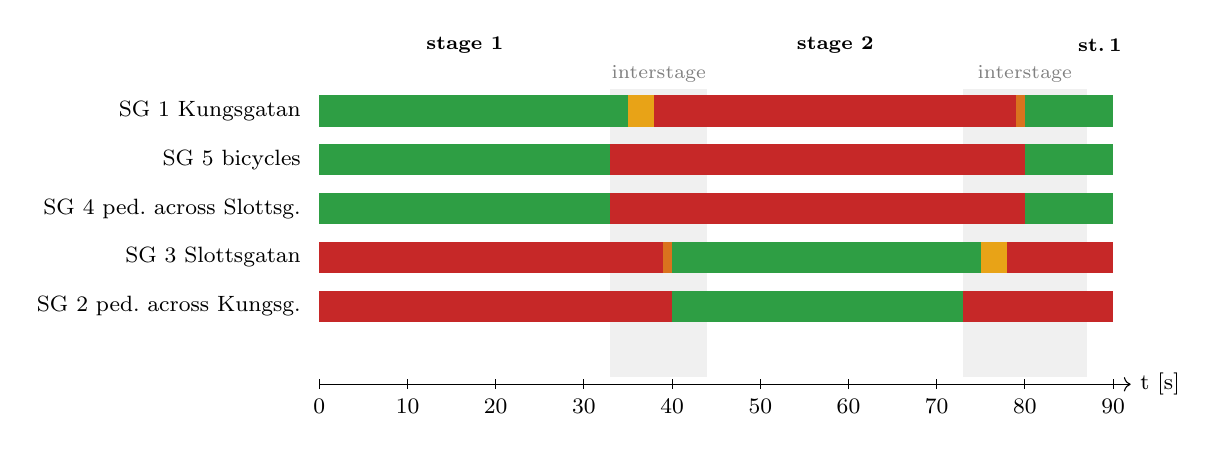
\begin{tikzpicture}[x=0.112cm, y=0.62cm, font=\footnotesize]
  % helper: bar(row, from, to, color)
  \newcommand{\sbar}[4]{\fill[#4] (#2,#1-0.32) rectangle (#3,#1+0.32);}
  % axis
  \draw[->] (0,-0.6) -- (92,-0.6) node[right]{t [s]};
  \foreach \t in {0,10,...,90} {\draw (\t,-0.5) -- (\t,-0.7) node[below]{\t};}
  % interstage shading
  \fill[gray!12] (33,-0.45) rectangle (44,5.45);
  \fill[gray!12] (73,-0.45) rectangle (87,5.45);
  \node[font=\scriptsize, text=gray] at (38.5,5.75) {interstage};
  \node[font=\scriptsize, text=gray] at (80,5.75) {interstage};
  % row labels
  \node[anchor=east] at (-1,5) {SG 1 Kungsgatan};
  \node[anchor=east] at (-1,4) {SG 5 bicycles};
  \node[anchor=east] at (-1,3) {SG 4 ped.\ across Slottsg.};
  \node[anchor=east] at (-1,2) {SG 3 Slottsgatan};
  \node[anchor=east] at (-1,1) {SG 2 ped.\ across Kungsg.};
  % SG1: green 0-35, amber 35-38, red 38-79, red/amber 79-80, green 80-90
  \sbar{5}{0}{35}{sgreen} \sbar{5}{35}{38}{samber} \sbar{5}{38}{79}{sred} \sbar{5}{79}{80}{samber!60!sred} \sbar{5}{80}{90}{sgreen}
  % SG5 and SG4: green 0-33, red 33-80, green 80-90
  \sbar{4}{0}{33}{sgreen} \sbar{4}{33}{80}{sred} \sbar{4}{80}{90}{sgreen}
  \sbar{3}{0}{33}{sgreen} \sbar{3}{33}{80}{sred} \sbar{3}{80}{90}{sgreen}
  % SG3: red 0-39, red/amber 39-40, green 40-75, amber 75-78, red 78-90
  \sbar{2}{0}{39}{sred} \sbar{2}{39}{40}{samber!60!sred} \sbar{2}{40}{75}{sgreen} \sbar{2}{75}{78}{samber} \sbar{2}{78}{90}{sred}
  % SG2: red 0-40, green 40-73, red 73-90
  \sbar{1}{0}{40}{sred} \sbar{1}{40}{73}{sgreen} \sbar{1}{73}{90}{sred}
  % stage labels
  \node[font=\scriptsize\bfseries] at (16.5,6.35) {stage 1};
  \node[font=\scriptsize\bfseries] at (58.5,6.35) {stage 2};
  \node[font=\scriptsize\bfseries] at (88.5,6.35) {st.\,1};
\end{tikzpicture}
\caption[Fixed-time signal plan]{Fixed-time signal plan (program 1, cycle 90~s) as read from
\code{Fixed\_time.sig}. Green, amber and red bars show the signal colour; grey shading marks the two
interstages.}
\label{fig:timing}
\end{figure}

\begin{table}[!htb]
\centering
\caption[Green times per cycle]{Green times per 90~s cycle, read from the signal program.}
\label{tab:green}
\small
\begin{tabular}{lrrr}
\toprule
\textbf{Signal group} & \textbf{Green} & \textbf{Amber} & \textbf{Share of cycle}\\
\midrule
Kungsgatan vehicles (SG 1)              & 45~s & 3~s & 53\,\%\\
Slottsgatan vehicles (SG 3)             & 35~s & 3~s & 42\,\%\\
Bicycles, pedestrians across Slottsgatan (SG 5, 4) & 43~s & & 48\,\%\\
Pedestrians across Kungsgatan (SG 2)    & 33~s & & 37\,\%\\
\bottomrule
\end{tabular}
\end{table}

The signal file also contains a second program (``Stage 1, Stage 2, Opt'') that shortens the
Slottsgatan stage by 10~s; it is not used in the model.

\begin{plainbox}{How busy is the busiest approach? (estimate)}
A single urban lane can discharge roughly 1\,800 to 1\,900 vehicles per hour of green (a typical
\emph{saturation flow}; this value is an assumption, not a number from the file). Kungsgatan
northbound has 45~s of green plus 3~s of amber out of 90~s, so its capacity is roughly
\[
1\,900 \cdot \frac{45 \text{ to } 48}{90} \approx 950 \text{ to } 1\,010 \text{ vehicles per hour}.
\]
The vehicles that stay in the main lane (straight and right, $780 + 177 = 957$ per hour) therefore
use 95 to 100\,\% of the capacity. This approach is \emph{near saturation}: small changes in driver
behaviour or demand can create long queues. All other approaches have plenty of spare capacity.
\end{plainbox}

\subsection{The actuated alternative}
\label{sec:actuated}

The lab also provides an \emph{actuated} controller, written in the VisVAP language
(\code{Control\_logic.vap}) together with the interstage definitions in \code{Signal\_data.pua}. It
uses the same two stages and the same interstages, but the length of each stage depends on the
traffic detected. Eight detectors, each 3~m long, are placed on the approaches and in the pockets
and send their signals to six input channels (\cref{tab:detectors}).

\begin{table}[!htb]
\centering
\caption[Detectors]{Detectors used by the actuated controller.}
\label{tab:detectors}
\small
\begin{tabular}{rllrr}
\toprule
\textbf{Det.} & \textbf{Link} & \textbf{Location} & \textbf{Channel} & \textbf{Distance to stop line}\\
\midrule
1 & 2  & Kungsgatan northbound, main lane     & 4 & 26~m\\
2 & 6  & Kungsgatan northbound, left pocket   & 5 & 4~m\\
4 & 4  & Kungsgatan southbound, main lane     & 1 & 26~m\\
3 & 8  & Kungsgatan southbound, left pocket   & 2 & 4~m\\
6 & 5  & Slottsgatan westbound, main lane     & 3 & 4~m\\
5 & 7  & Slottsgatan westbound, left pocket   & 3 & 4~m\\
7 & 11 & Slottsgatan eastbound, main lane     & 6 & 4~m\\
8 & 12 & Slottsgatan eastbound, left pocket   & 6 & 4~m\\
\bottomrule
\end{tabular}
\end{table}

The logic is evaluated once per second and follows the decision chart in \cref{fig:vap}. Stage 1
(Kungsgatan) is \emph{extended} as long as vehicles keep arriving on any Kungsgatan channel with a
time gap of at most 3~s, up to 75~s. When the gaps become longer, or the maximum is reached, the
controller switches to Slottsgatan only if a vehicle is waiting there (a \emph{call} on channel 3 or
6); otherwise Kungsgatan simply keeps green. Stage 2 (Slottsgatan) is extended in the same way but
for at most 15~s, and then the controller returns to Kungsgatan.

\begin{figure}[!htb]
\centering
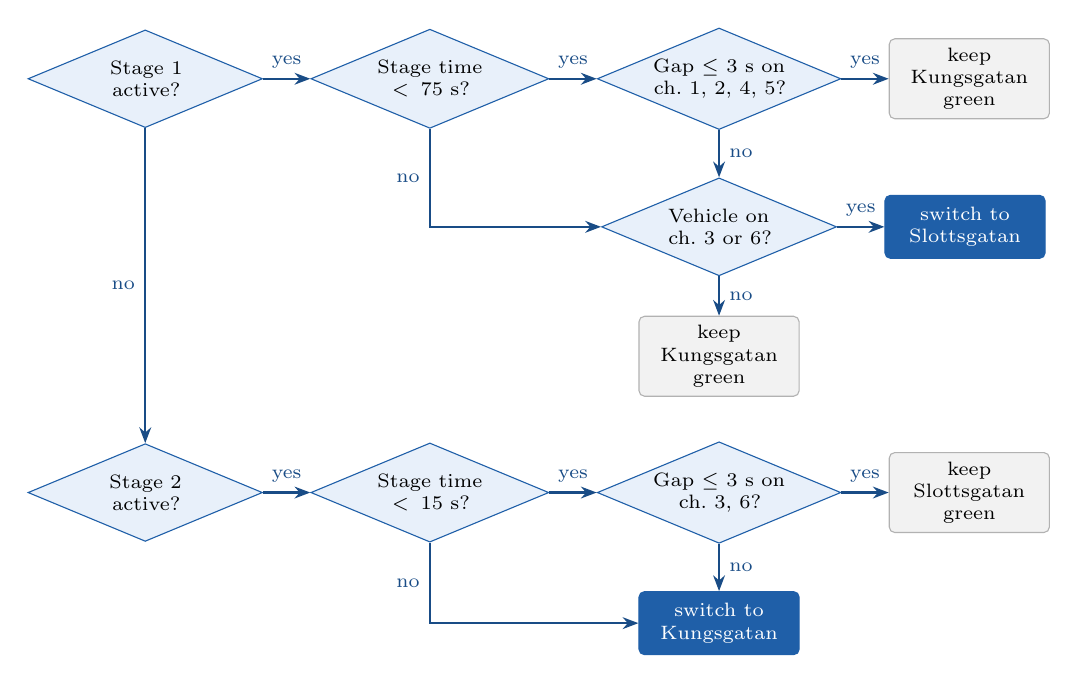
\begin{tikzpicture}[
  node distance=5mm and 6mm, font=\scriptsize,
  dec/.style={draw=accent, fill=lightaccent, diamond, aspect=2.4, inner sep=0pt, align=center, text width=19mm},
  act/.style={draw=accent, fill=accent, text=white, rounded corners=2pt, align=center, text width=18mm, minimum height=8mm},
  stay/.style={draw=gray!60, fill=gray!10, rounded corners=2pt, align=center, text width=18mm, minimum height=8mm},
  arr/.style={-{Stealth[length=2mm]}, thick, accent!80!black}]
% stage 1 branch
\node[dec] (s1) {Stage 1\\active?};
\node[dec, right=of s1] (m1) {Stage time\\$< 75$~s?};
\node[dec, right=of m1] (e1) {Gap $\le 3$~s on\\ch.\ 1, 2, 4, 5?};
\node[stay, right=of e1] (k1) {keep\\Kungsgatan green};
\node[dec, below=6mm of e1] (c2) {Vehicle on\\ch.\ 3 or 6?};
\node[act, right=of c2] (i12) {switch to\\Slottsgatan};
\node[stay, below=5mm of c2] (k1b) {keep\\Kungsgatan green};
% stage 2 branch
\node[dec, below=40mm of s1] (s2) {Stage 2\\active?};
\node[dec, right=of s2] (m2) {Stage time\\$< 15$~s?};
\node[dec, right=of m2] (e2) {Gap $\le 3$~s on\\ch.\ 3, 6?};
\node[stay, right=of e2] (k2) {keep\\Slottsgatan green};
\node[act, below=6mm of e2] (i21) {switch to\\Kungsgatan};
\draw[arr] (s1) -- node[above]{yes} (m1);
\draw[arr] (m1) -- node[above]{yes} (e1);
\draw[arr] (e1) -- node[above]{yes} (k1);
\draw[arr] (e1) -- node[right]{no} (c2);
\draw[arr] (m1) |- node[pos=0.25, left]{no} (c2);
\draw[arr] (c2) -- node[above]{yes} (i12);
\draw[arr] (c2) -- node[right]{no} (k1b);
\draw[arr] (s1) -- node[left]{no} (s2);
\draw[arr] (s2) -- node[above]{yes} (m2);
\draw[arr] (m2) -- node[above]{yes} (e2);
\draw[arr] (e2) -- node[above]{yes} (k2);
\draw[arr] (e2) -- node[right]{no} (i21);
\draw[arr] (m2) |- node[pos=0.25, left]{no} (i21);
\end{tikzpicture}
\caption[Logic of the actuated controller]{Logic of the actuated controller, simplified from
\code{Control\_logic.vap}. The check runs once per second; during an interstage nothing is decided.}
\label{fig:vap}
\end{figure}

%=====================================================================
\section{What the model measures}
\label{sec:measure}
%=====================================================================

The model contains three kinds of measurement objects, which record what happens during a run.

\subsection{Data collection points: speeds and accelerations}

A \emph{data collection point} works like a loop detector in the road: it records every vehicle
that passes and its speed and acceleration at that moment. The model has twelve, called L1 to L12,
at the same places where the field data were collected (\cref{tab:dc}). The position relative to
the stop line decides what a point actually sees: points shortly before a stop line see vehicles
braking or queueing, points after the junction see vehicles accelerating away.

\begin{table}[!htb]
\centering
\caption[Data collection points]{The twelve data collection points (Vissim data collection
measurements 1 to 12) and what they mainly capture.}
\label{tab:dc}
\small
\begin{tabularx}{\textwidth}{llllX}
\toprule
\textbf{Point} & \textbf{Name in the model} & \textbf{Link} & \textbf{Position} & \textbf{Mainly captures}\\
\midrule
L1  & Slottsgatan\_East\_in   & 5  & 14.0~m before stop line & braking and queueing; straight and right only\\
L2  & Slottsgatan\_West\_out  & 3  & 34~m along the exit     & acceleration after the junction\\
L3  & Kungsgatan\_South\_out  & 4  & 52.6~m after stop line  & acceleration towards desired speed\\
L4  & Kungsgatan\_South\_in   & 2  & 11.7~m before stop line & queue on the busiest approach\\
L5  & Slottsgatan\_East\_out  & 1  & 19~m along the exit     & acceleration after the junction\\
L6  & Kungsgatan\_North\_out  & 2  & 55.3~m after stop line  & acceleration towards desired speed\\
L7  & Kungsgatan\_North\_in   & 4  & 2.1~m \emph{after} stop line & discharge from the stop line\\
L8  & Slottsgatan\_West\_in   & 11 & 4.1~m before stop line  & braking and queueing; straight and right only\\
L9 to L12 & Kungsgatan bike points & 19 to 22 & on the cycle tracks & cyclist speeds\\
\bottomrule
\end{tabularx}
\end{table}

Because left-turners leave the main lane into the pocket before L1, L4, L7 and L8, these points see
only straight and right-turning vehicles. At L1 and L8 most of them are right-turners
($101/120 = 84\,\%$ and $61/90 = 67\,\%$), so the right-turn speed strongly influences these points.

\subsection{Queue counters}

A \emph{queue counter} measures the length of the queue upstream of its position. A vehicle is
counted as queueing when its speed falls below 5\kmh{} and stops being counted when it exceeds
10\kmh{}; vehicles more than 20~m apart are not considered part of the same queue, and queues are
followed up to 500~m. The model has ten queue counters: one at each of the eight vehicle stop lines
(main lane and left pocket of every approach) and one on each cycle track. They report the average
queue length, the maximum queue length and the number of stops in the queue.

\subsection{Vehicle network performance}

This evaluation summarises the whole network in a few numbers, most importantly the \emph{average
delay per vehicle}. The delay of a trip is its actual travel time minus the travel time it would
have had without other vehicles, signals or stops. Average delay is the usual measure of the
\emph{level of service} of a signalised intersection. The same evaluation also gives the number of
stops per vehicle, the average speed and the number of vehicles that completed their trip.

%=====================================================================
\section{Running the model}
\label{sec:running}
%=====================================================================

\Cref{tab:sim} lists the simulation settings stored in the original file.

\begin{table}[!htb]
\centering
\caption[Simulation settings]{Simulation settings of the original model file.}
\label{tab:sim}
\small
\begin{tabularx}{\textwidth}{lrX}
\toprule
\textbf{Setting} & \textbf{Value} & \textbf{Meaning}\\
\midrule
Simulation period & 1\,800~s & 30 minutes of traffic are simulated.\\
Simulation resolution & 10 & Time steps per simulated second (step of 0.1~s).\\
Number of runs & 5 & Replications performed one after another.\\
Random seed & 42 & Starting value of the random number generator.\\
Random seed increment & 1 & Each following run uses the next seed (42, 43, 44, \dots).\\
Evaluation interval & 0 to 1\,800~s & Results are aggregated over the whole period.\\
\bottomrule
\end{tabularx}
\end{table}

\paragraph{Warm-up.} At the start of a run the network is empty. During the first minutes there are
fewer vehicles and shorter queues than in normal operation. In the original file the measurements
start at second 0, so this unrealistic start-up phase is included in the results. In the
calibration work (\cref{sec:calibration}) the period was extended to 2\,400~s and the first 600~s
were excluded as \emph{warm-up}.

\paragraph{How many runs?} Because every run is one random outcome, the mean of several runs is
used. The number of runs $n$ needed for a mean $\bar x$ with relative accuracy $\varepsilon$ follows
the course formula
\begin{equation}
n = \left(\frac{t_{0.975,\,n_0-1}\; s}{\varepsilon\, \bar x}\right)^2,
\end{equation}
where $s$ is the standard deviation between $n_0$ pilot runs and $t$ the Student $t$ value. For
$\varepsilon = 5\,\%$ the points after the junction need only one or two runs, but the low-speed
approach points L1 and L8 need about 10 to 14 runs, because few vehicles pass them and their speed
depends on whether they arrive on red or green.

%=====================================================================
\section{Is the model realistic? Field data and calibration}
\label{sec:calibration}
%=====================================================================

\subsection{The field data}

The file \code{traffic\_measurements.xlsx} contains the mean speed at L1 to L12 and the mean
acceleration at L1 to L8, measured on ten weekday mornings under the current fixed-time control
and the current demand. A model is accepted at a point if a two-sample $t$-test (95\,\% confidence)
cannot distinguish the simulated mean from the field mean. The measured variation between days is
very different between points: the standard deviation of the mean speed is 4.7\kmh{} at L1 but
only 0.3\kmh{} at L3.

\subsection{How well the original model fits}

With a 600~s warm-up and ten replications, the original model reproduces the accelerations well
(7 of 8 points pass the test) but only 2 of the 12 speeds. The main differences have clear causes
in the model mechanics described above:
\begin{itemize}
  \item \textbf{L1 and L8 are too fast} (by 10.7 and 4.7\kmh): most vehicles there turn right, but
        the reduced speed areas lie after the stop line (\cref{sec:rsa}), so they pass the
        measurement point almost at full speed.
  \item \textbf{L4 and L7 are too fast} (by about 5\kmh): approach speed and queue discharge on
        Kungsgatan are higher than observed.
  \item \textbf{Cyclists are too slow} (by about 3.8\kmh): the model's mean desired speed is
        $0.8 \cdot 13.5 + 0.2 \cdot 17.5 = 14.3$\kmh, while about 18\kmh{} is observed.
\end{itemize}

\subsection{The calibrated model}

The model was calibrated automatically: Python generated hundreds of model variants with different
parameter values, ran them in Vissim, learned a statistical \emph{surrogate model} (a Gaussian
process) that predicts the results from the parameters, and used it to find the best parameter
values, which were then checked with new random seeds. The recommended calibrated model changes the
parameters in \cref{tab:calib}.

\begin{table}[!htb]
\centering
\caption[Original and calibrated parameters]{Original and calibrated parameter values
(recommended model).}
\label{tab:calib}
\small
\begin{tabularx}{\textwidth}{lrrX}
\toprule
\textbf{Parameter} & \textbf{Original} & \textbf{Calibrated} & \textbf{Interpretation}\\
\midrule
Bicycle / e-bike desired speed & 13.5 / 17.5 & 17.3 / 21.3 & cyclists ride faster than assumed\\
Right-turn speed (cars) & 22.5 & 10.1 & right turns are taken slowly\\
Left-turn speed (cars) & (27.5) & 29.9 & now defined on all left turns\\
Desired speed Slottsgatan from the east & 53 & 43.9 & a slower street than the others\\
Desired speed other approaches & 53 & 51.3 to 52.4 & close to the original\\
$a_x$ / $b_{x,\mathrm{add}}$ / $b_{x,\mathrm{mult}}$ & 2.0 / 2.0 / 3.0 & 1.49 / 0.82 / 1.39 & tighter following keeps the busy approach at capacity\\
Reduction factor near signals & 0.6 & 0.31 & drivers close up more near the stop line\\
Desired acceleration / deceleration scale & 1.0 / 1.0 & 1.04 / 0.89 & almost unchanged\\
\bottomrule
\end{tabularx}
\smallskip

{\footnotesize Speeds in km/h, centre of a uniform distribution. Each motorised input received its
own desired speed distribution.}
\end{table}

With these values the average speed error over the twelve points falls from 4.53 to 2.01\kmh, the
acceleration error stays at the original level (0.13~m/s$^2$), all four cycle-track points and the
points L6, L7 and L8 pass the test (10 of 20 tests in total), and the full demand is still served.
\Cref{fig:residuals} compares the original and the calibrated model point by point.

\begin{figure}[!htb]
\centering
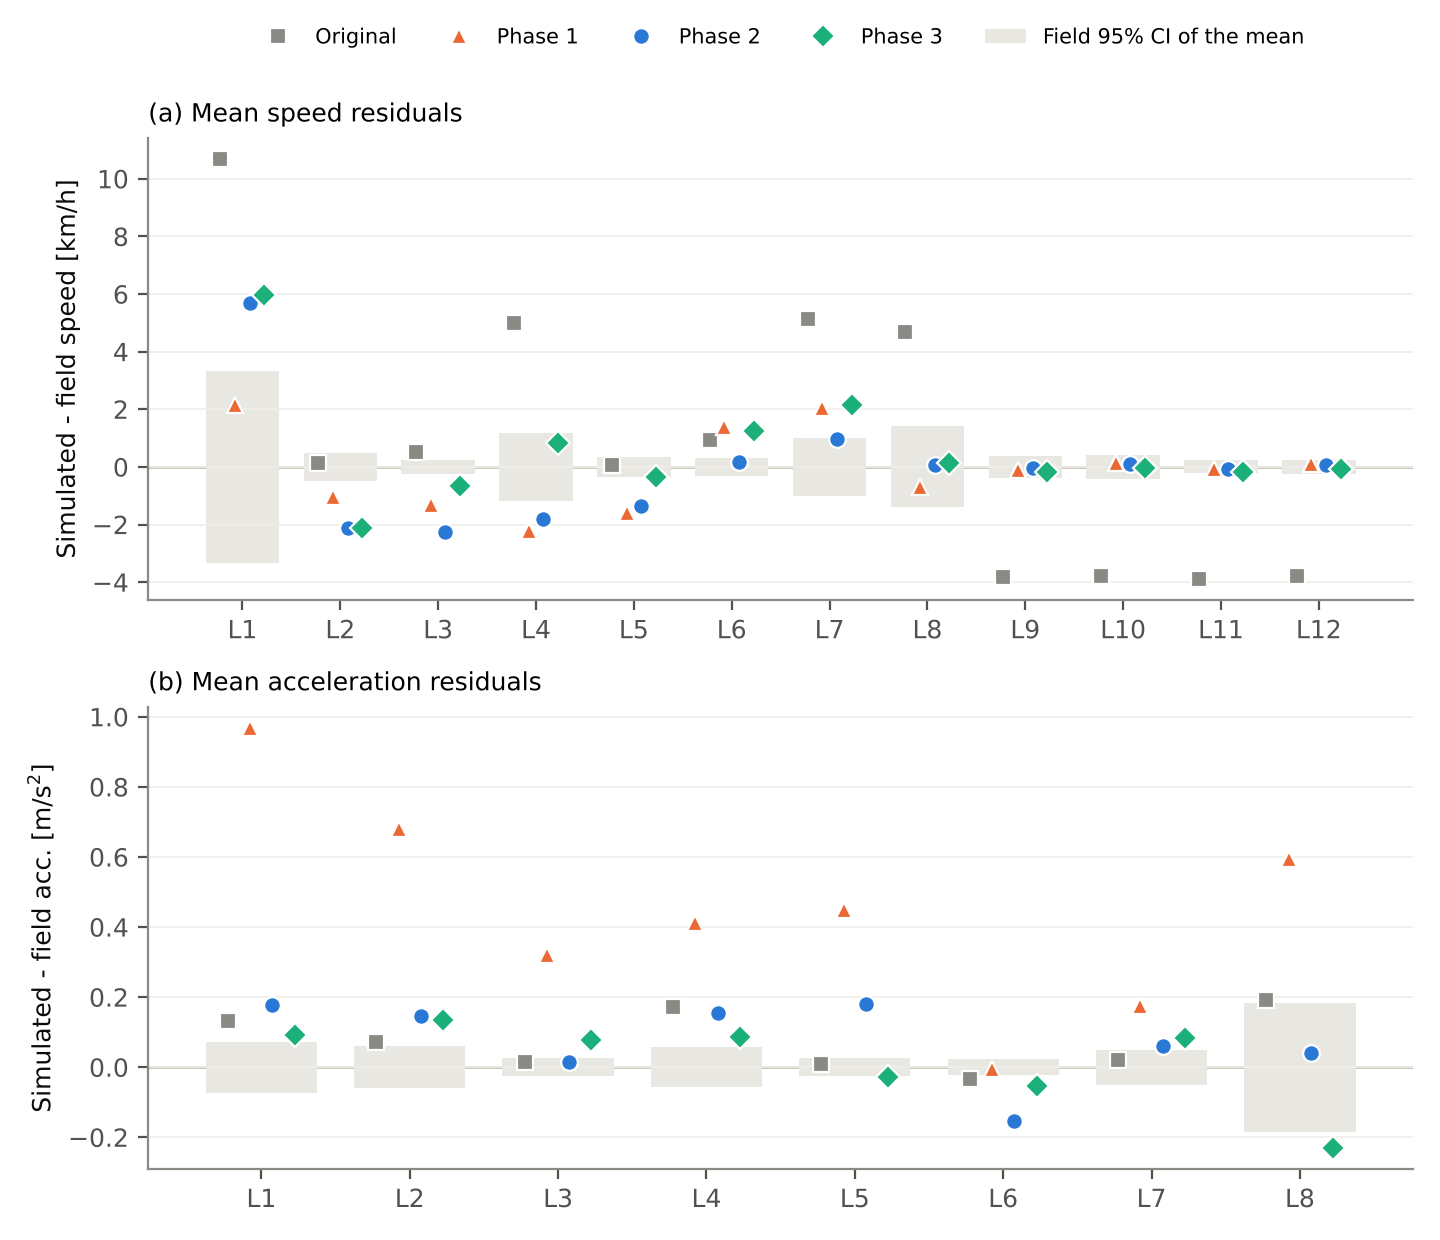
\includegraphics[width=\textwidth]{fig_residuals.png}
\caption[Simulated minus field values]{Simulated minus field mean for (a) speeds and (b)
accelerations, ten independent runs. The grey bars show the 95\,\% confidence interval of the field
mean. The phase 2 model is the recommended calibrated model.}
\label{fig:residuals}
\end{figure}

\subsection{What the calibrated model was used for}

The calibrated model is the baseline for comparing designs under identical conditions (20 runs
each with the same random seeds). \Cref{tab:alt} summarises the three alternatives of the lab.

\begin{table}[!htb]
\centering
\caption[Results of the alternative designs]{Results of the alternative designs compared with the
calibrated baseline (average delay of all vehicles, 20 runs).}
\label{tab:alt}
\small
\begin{tabularx}{\textwidth}{lrX}
\toprule
\textbf{Scenario} & \textbf{Delay [s/veh]} & \textbf{What happens}\\
\midrule
Baseline (fixed time) & 21.3 & Reference.\\
Actuated control (\cref{sec:actuated}) & 15.7 & 26\,\% less delay: unused Slottsgatan green is
given to the near-saturated Kungsgatan; Kungsgatan queues are halved.\\
Incident demand (volumes change every 10 min) & 21.3 & No change on average, but Slottsgatan
left-turn queues double in minutes 10 to 20 and then dissolve.\\
800 bicycles per hour and direction & 22.5 & Right-turning cars wait for cyclists; car flow on
Kungsgatan drops by 7\,\% and stops double.\\
\bottomrule
\end{tabularx}
\end{table}

%=====================================================================
\section{Simplifications and limitations}
\label{sec:limits}
%=====================================================================

The lab instructions state that the model is a simplification of reality made for teaching. A
reader should keep the following points in mind:
\begin{itemize}
  \item Each approach has one lane plus a left-turn pocket; there are no gradients, parking, buses or
        other intersections nearby.
  \item The demand is constant over the half hour and there are no field counts of traffic volume,
        so the demand is taken as given.
  \item Pedestrians are modelled as a simple vehicle type that walks without interacting with other
        pedestrians, and all of them are of the type ``Man''.
  \item Turning speeds act only on the connectors, i.e.\ after the stop line, and three of the four
        left-turn areas have no speed in the original file (\cref{sec:rsa}).
  \item The original file has no warm-up period, which biases results towards an emptier network.
  \item The model is calibrated for 100 cyclists per hour; results far outside this situation, such as
        800 cyclists per hour, are less certain because the car and cyclist interaction could not be
        calibrated with the available data.
\end{itemize}

%=====================================================================
\section{Glossary}
\label{sec:glossary}
%=====================================================================

\begin{description}[style=nextline, leftmargin=1.2cm, font=\bfseries\color{accent}]
  \item[Calibration] Adjusting model parameters until simulated results agree with field
        measurements.
  \item[Capacity] The largest number of vehicles that can pass a point per hour.
  \item[Conflict area] An area where two paths cross or merge, with a rule for who goes first.
  \item[Connector] A short link piece that joins two links; all turns are connectors.
  \item[Cycle time] Time for one complete sequence of all signal stages (here 90~s).
  \item[Data collection point] A virtual detector that records passing vehicles, their speed and
        acceleration.
  \item[Delay] Actual travel time minus the travel time without other traffic, signals or stops.
  \item[Desired speed] The speed a road user would choose on an empty road.
  \item[Detector] A sensor in the road that tells an actuated controller that a vehicle is present.
  \item[Interstage] The transition between two signal stages, with amber and clearance time.
  \item[Link] A directed road section with one or more lanes.
  \item[Queue counter] An object that measures the length of the queue upstream of it.
  \item[Random seed] Starting value for the random numbers; the same seed gives the same run.
  \item[Reduced speed area] A section where road users temporarily use a lower desired speed,
        e.g.\ in a turn.
  \item[Replication (run)] One simulation of the period with one random seed.
  \item[Saturation flow] The rate at which a queue discharges during green, in vehicles per hour of
        green.
  \item[Signal group] A set of signal heads that always show the same colour.
  \item[Stage] A combination of signal groups that have green at the same time.
  \item[Surrogate model] A fast statistical model that imitates the results of the slow simulation.
  \item[Vehicle composition] The mix of vehicle types arriving at an input.
  \item[Vehicle input] The point where road users enter the network, with a volume per hour.
  \item[Warm-up] The initial part of a run that is not evaluated, because the network starts empty.
  \item[Wiedemann 74 / 99] Car-following models in Vissim that describe how a driver follows the
        vehicle in front.
\end{description}

%=====================================================================
\appendix
\section{Where to find each element in Vissim}
\label{app:where}
%=====================================================================

\begin{table}[!htb]
\centering
\caption[Model elements and where to find them in Vissim]{Model elements described in this
document and where to find them in the Vissim user interface.}
\label{tab:where}
\small
\begin{tabularx}{\textwidth}{lX}
\toprule
\textbf{Element} & \textbf{Vissim menu or object}\\
\midrule
Links and connectors & Network objects sidebar: Links\\
Vehicle inputs & Network objects sidebar: Vehicle Inputs, show list\\
Routes & Network objects sidebar: Vehicle Routes, Static, show list\\
Vehicle compositions & Traffic: Vehicle Compositions\\
Desired speed distributions & Base Data: Distributions: Desired Speed\\
Acceleration functions & Base Data: Distributions (acceleration and deceleration functions)\\
Car-following parameters & Base Data: Driving Behaviors: Urban (motorized)\\
Reduced speed areas & Network objects sidebar: Reduced Speed Areas\\
Conflict areas & Network objects sidebar: Conflict Areas\\
Signal controller & Signal Control: Signal Controllers (VISSIG editor for \code{Fixed\_time.sig})\\
Detectors & Network objects sidebar: Detectors\\
Data collection points & Network objects sidebar: Data Collection Points; Evaluation: Measurement
Definition: Data Collection Measurements\\
Queue counters & Network objects sidebar: Queue Counters\\
Simulation settings & Simulation: Parameters\\
Evaluation settings & Evaluation: Configuration: Result Attributes\\
\bottomrule
\end{tabularx}
\end{table}

\end{document}
